\documentclass[conference]{IEEEtran}
\usepackage{graphicx}
\usepackage{tikz}
 
\usepackage[colorlinks = true, citecolor = blue]{hyperref}

% math lib
\usepackage{amsmath}
\usepackage{mathrsfs}

% operators
\DeclareMathOperator*{\argmax}{arg\,max}
\DeclareMathOperator*{\argmin}{arg\,min}
\newcommand\ceiling[1]{\left\lceil #1 \right\rceil}

% empty set
\usepackage{amssymb}
\let\emptyset=\varnothing

% algorithms
\usepackage{algorithm}
\usepackage{algorithmic}
\renewcommand{\algorithmicrequire}{\textbf{Input:}}
\renewcommand{\algorithmicensure}{\textbf{Output:}}

\begin{document}
% --------------------------------------------
% --------------Change HERE! -----------------
% --------------------------------------------
\def\authorone{Jaesung Yoo}
\def\authortwo{Soham Choudhury}
\def\groupid{6}
% --------------------------------------------
\title{CS258 Final Report: The RSA Problem}
\author{
    \IEEEauthorblockN{\authorone\ and \authortwo}
    \IEEEauthorblockA{
        Group \groupid
    }    
}

\maketitle
\IEEEpeerreviewmaketitle


\section{Methods: Routing using Reinforcement Learning}
\subsection{Reinforcement Learning Algorithms}
% List RL algorithms and give a brief explanation of each
\subsubsection{PPO}
The first Reinforcement Learning (RL) algorithm that was used is PPO [1], which is shortened for Proximal Policy Optimization. PPO is one of the most commonly used RL algorithms. It learns on-policy which means it updates the policy of each stage based on the data collected by the current policy during training. PPO focuses on balancing between improving the policy and avoiding large updates which stabilizes learning.

\subsubsection{DQN}
The second RL algorithm that was used is DQN algorithm [2], which is shortened for Deep Q-Network. DQN is widely used in games as it is estimates the expected total long term reward when traveling through an optimal policy. It first initializes an empty neural network, then travels randomly, stores the results (rewards), then learns from those results.

The main difference between the two RL algorithms is that PPO is a policy-based algorithm which comes up with a policy function. On the other hand, DQN is a value-based algorithm which learns a Q-function to estimate the expected future rewards when taking the next action.


\subsection{State Space}
% Explain state/action/reward
% Make sure you provide enough information to reconstruct results
% Check https://gymnasium.farama.org/environments/box2d/lunar_lander/ for some examples
The state space includes links for each edge in the graph and request. The capacity for all edges is set to 10 links.

Each request includes the following:
\begin{itemize}
    \item Source
    \item Destination
    \item Holding Time
\end{itemize}

\subsection{Action Space}
There are 4 actions available for the agent to take:
\begin{itemize}
    \item 0: Choose Path 1
    \item 1: Choose Path 2
    \item 2: Choose Path 3
    \item 3: Blocking action
\end{itemize}
\subsection{Reward Function}
After every step a reward is granted. The return of an episode is the sum of the rewards for all the steps within that episode.

For each step, the reward is either:
\begin{itemize}
    \item -1 if the request is blocked.
    \item the value of the holding time of the request if it is accommodated.
\end{itemize}

The maximum expected mean return is 1,500 if there is no block because the reward is chosen randomly between 10 and 20 which repeats for 100 requests. However, this is highly unlikely as there will be blocks happening as there are 100 requests and the return will decrease by 1 whenever one of them is blocked.

\section{Method: Spectrum Allocation}
% Explain your heuristic
% If you have multiple, you can make subsections 
\subsubsection{Simple Heuristic Algorithm: Shortest Path Sequential Spectrum Allocation}
Sequential Spectrum Allocation algorithm follows an approach of assigning the first available spectrum slot that can accommodate the request.
The steps of the Sequential Spectrum Allocation are as follows:

Given the shortest path between a request's source and destination, iterate over each edge in the path.
For each edge, find the first available spectrum slot that is not currently in use.
If an available slot is found on all edges of the path, assign the request to that spectrum slot by allocating the holding time of the request for each edge.
If no available slot is found on at least one edge of the path, the request is blocked.

The key advantage of the Sequential Spectrum Allocation is that it requires minimal computations to find the first available spectrum slot as it aims to allocate spectrum slots efficiently by assigning requests to the first available slot that can accommodate them. It takes into account factors such as link capacities and the current utilization of spectrum slots on each edge.

One potential drawback of the Shortest Path Sequential Spectrum Allocation is that it may lead to inefficient use of the spectrum over time. Since the algorithm always assigns requests to the same path, it does not consider the long-term impact of these assignments on future requests. This can potentially reduce the overall spectrum utilization across all edges in the network and increase the blocking probability for future requests.
% If you borrow some ideas from papers, cite them with bibtex (e.g. \cite{8509143})


\section{Results}
\subsection{Learning Curve}
% Insert figures
% Explain the results
x-axis represents the number of timesteps. y-axis represents the return from an episode of a hundred rounds. The graphs were visualized using TensorBoard. 

\begin{figure}[h]
    \centering
    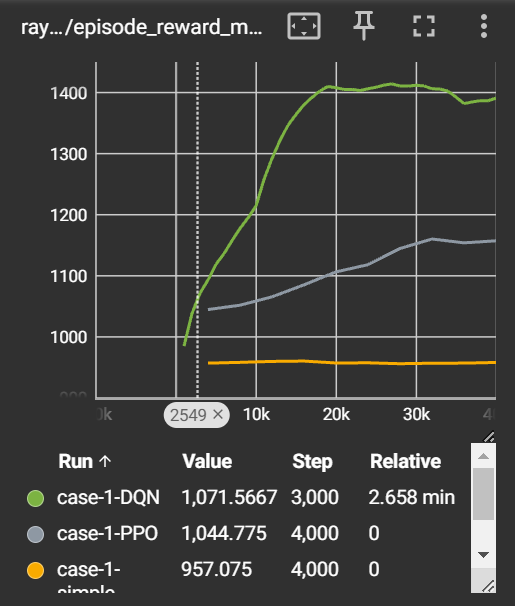
\includegraphics[width=0.75\linewidth]{all1.png}
    \caption{Case1-Total}
    \label{fig:enter-label}
\end{figure}

\subsubsection{Case 1}
All requests have the same source and destination pair which were \textit{San Diego Supercomputer Center} to \textit{Jon Von Neumann Center, Princeton, NJ}, respectively.


The results for Case 1 indicate that the DQN method exhibited the best performance among the compared approaches. Although PPO also demonstrated a learning curve, its performance improvement was not as substantial as that of DQN. 

The simple shortest path algorithm did not show any performance improvement over time. This is because the shortest path algorithm does not incorporate any learning mechanism and, therefore, cannot learn from its experiences to adapt and optimize its decision-making process.

\subsubsection{Case 2}
\begin{figure}[h]
    \centering
    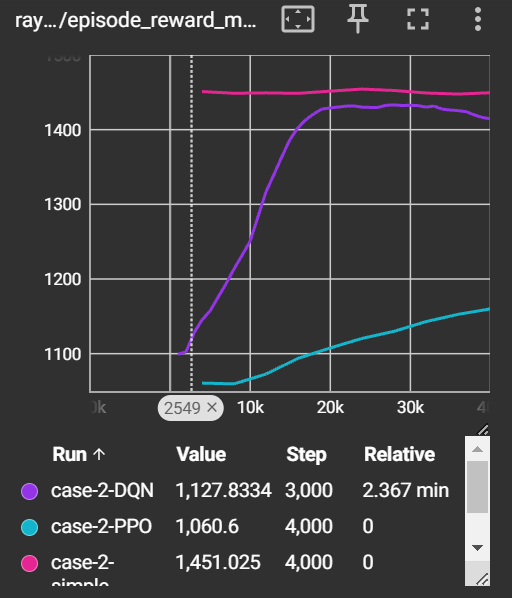
\includegraphics[width=0.75\linewidth]{all2.png}
    \caption{Case2-Total}
    \label{fig:enter-label}
\end{figure}

The source and destination nodes are selected uniform-randomly among all nodes. Source and destination are not equal.

The results for Case 2 demonstrate that both DQN and PPO exhibited learning curves, indicating their ability to improve performance over time. However, DQN significantly outperformed PPO, showing a dramatic enhancement in performance as the training progressed. Interestingly, the simple shortest path algorithm achieved the best results in this case. This is because the shortest path algorithm consistently chooses edges from the same path, leading to faster saturation of links on those edges and, consequently, increased blocking. However, our implementation considers three disjoint paths for every source-destination pair, allowing for better distribution of traffic and potentially reducing the likelihood of blocking in case one or more of the ten links in each edge goes offline.
\subsection{Utilization (The Objective)}
 The primary objective of spectrum allocation is to efficiently assign available spectrum slots to the requests while minimizing the overall blocking probability and maximizing the network utilization.

 Spectrum utilization increased when using the RL algorithms because the increase in performance over time for both algorithms represent that there were more successes from source to destination compared to the previous episodes. It also demonstrates that the blocking probability has decreased over time as they learned.
\subsection{Comparison}
For both cases, both RL algorithms, PPO and DQN successfully demonstrated their learning curves through the results above. The simple shortest path algorithm did not show its learning curve which was expected as it does not learn from any of its past experiences. In Case 1, the results derived from the simple shortest path algorithm performed poorly compared to the RL-based algorithms. However, in Case 2, the simple shortest path algorithm performed almost equally to the DQN-trained RL agent. This is because the same few edges that were being used in Case 1 are no longer facing a high load of requests. In both versions, the Simple Heuristic Algorithm and the RL-based algorithms, the requests are now being accommodated by edges belonging to various paths. It can be reasonably inferred that if the number of links belonging to each edge in the network was decreased to a lower value than the current value of ten, then we will again see the RL-based algorithms outperforming the Simple Heuristic Algorithm.

The results clearly indicated that DQN learned much better compared to PPO. For case 2, DQN reached reward value over 1,400 after 40,000 timestamps, whereas PPO reached only around 1100 after 80,000 timestamps. This applies the same for both Cases 1 and 2, meaning it is regardless of the randomness of source and destination

\bibliography{ref}
\bibliographystyle{ieeetr}
[1] OpenAI, "Proximal Policy Optimization", openai.com
https://openai.com/index/openai-baselines-ppo

\noindent [2] OpenAI, "OpenAI Baselines: DQN", openai.com
https://openai.com/index/openai-baselines-dqn
\end{document}



